
The $\sqrt{3}$ subdivision scheme was introduced by
Kobbelt~\cite{sqrt3}. It is an adaptive scheme, but in our example
progra we realize only a single uniform subdivision step.

The subdivision step takes a triangle mesh as input and splits each
facet at its centroid into three triangles.  We write a function that
creates the centroid for one triangle. The combinatorial part exists
already as an Euler operator for \cgalpoly, only the coordinates of
the new vertex need to be computed. We exploit the knowledge that the
facet is a triangle and access the 1-ring of the centroid directly
without any loops or branching decisions.

\begin{lstlisting}
void create_centroid( Polyhedron& P, Facet_iterator f) {
    Halfedge_handle h = f->halfedge();
    Vector vec = h->vertex()->point() - CGAL::ORIGIN;
    vec = vec + (h->next()->vertex()->point() - CGAL::ORIGIN);
    vec = vec + (h->next()->next()->vertex()->point() - CGAL::ORIGIN);
    Halfedge_handle new_center = P.create_center_vertex( h);
    new_center->vertex()->point() = CGAL::ORIGIN + (vec / 3.0);
}
\end{lstlisting}

We could instead generalize the method to allow non-triangular facets
in the first step. We would need to to replace the centroid
computation with a loop based on a circulator over the halfedges
surrounding the facet. Circulators are the corresponding concept for
circular sequences as iterator are the concept for linear sequences.
Main difference are the lack of a past-the-end position for
circulators that leads to the typical ideom of a do-while-loop instead
of the usual while-loop for iterators. The example loop could like this
including the count for the facet size:

\begin{lstlisting}
    Halfedge_around_facet_circulator h = f->facet_begin();
    do {
        vec = vec + ( h->vertex()->point() - CGAL::ORIGIN);
        ++ facet_size;
    } while ( ++h != f->facet_begin());
\end{lstlisting}

Next, all edges of the initial mesh are flipped so that they join two
adjacent centroids. The edge flip is part of the \cgalpoly\ interface.

Finally, each initial vertex is replaced by a barycentric combination
of its neighbors. However, the mesh has already been subdivided, so
the original neighbors of a vertex are actually every other vertex in
the 1-ring. We write a function object for the smoothing step that
will be efficiently applicable with the \lstinline!std::transform!
function.

\begin{lstlisting}
struct Smooth_old_vertex {
Point operator()( const Vertex& v) const {
    std::size_t degree = v.vertex_degree() / 2;
    double alpha = (4.0 - 2.0 * cos( 2.0 * CGAL_PI / degree)) / 9.0;
    Vector vec = (v.point() - CGAL::ORIGIN) * ( 1.0 - alpha);
    Halfedge_around_vertex_const_circulator h = v.vertex_begin();
    do {
        vec = vec + ( h->opposite()->vertex()->point() - CGAL::ORIGIN) 
                   * alpha / degree;
        ++ h; ++ h;
    } while ( h != v.vertex_begin());
    return (CGAL::ORIGIN + vec);
}
};
\end{lstlisting}

We are ready to assemble the subdivision program. We are exloiting
that newly created items are appended at the end, so that we can keep valid
iterators that tell us where the old items end and where the new items
start. We use this to be as economical as possible with the extra
storage needed in this method, which is an extra array for the
smoothed coordinates of original vertices. We start by creating the
centroids, then smooth the old vertices, and conclude with flipping
the old edges.

\begin{lstlisting}
void subdiv( Polyhedron& P) {
    std::size_t nv = P.size_of_vertices();
    Vertex_iterator last_v = P.vertices_end();
    -- last_v;  // the last of the old vertices
    Edge_iterator last_e = P.edges_end();
    -- last_e;  // the last of the old edges
    Facet_iterator last_f = P.facets_end();
    -- last_f;  // the last of the old facets

    Facet_iterator f = P.facets_begin(); // centroids
    do {
        create_centroid( P, f);
    } while ( f++ != last_f);

    std::vector<Point> pts;              // smooth old vertices
    pts.reserve( nv);  // get intermediate space for the new points
    ++ last_v; // make it the past-the-end position again
    std::transform( P.vertices_begin(), last_v, std::back_inserter( pts), 
                    Smooth_old_vertex());
    std::copy( pts.begin(), pts.end(), P.points_begin());

    ++ last_e; // make it the past-the-end position again
    for ( Edge_iterator e = P.edges_begin(); e != last_e; ++e)
        P.flip_edge(e);    // flip the old edges
}
\end{lstlisting}



An example of one step of
the $\sqrt{3}$ subdivision scheme is shown in
Fig.\ref{fig:sqrt3_basic}, and an example of several steps is shown in
Fig.\ref{fig:sqrt3}.

\begin{figure}[htb]
    \centering{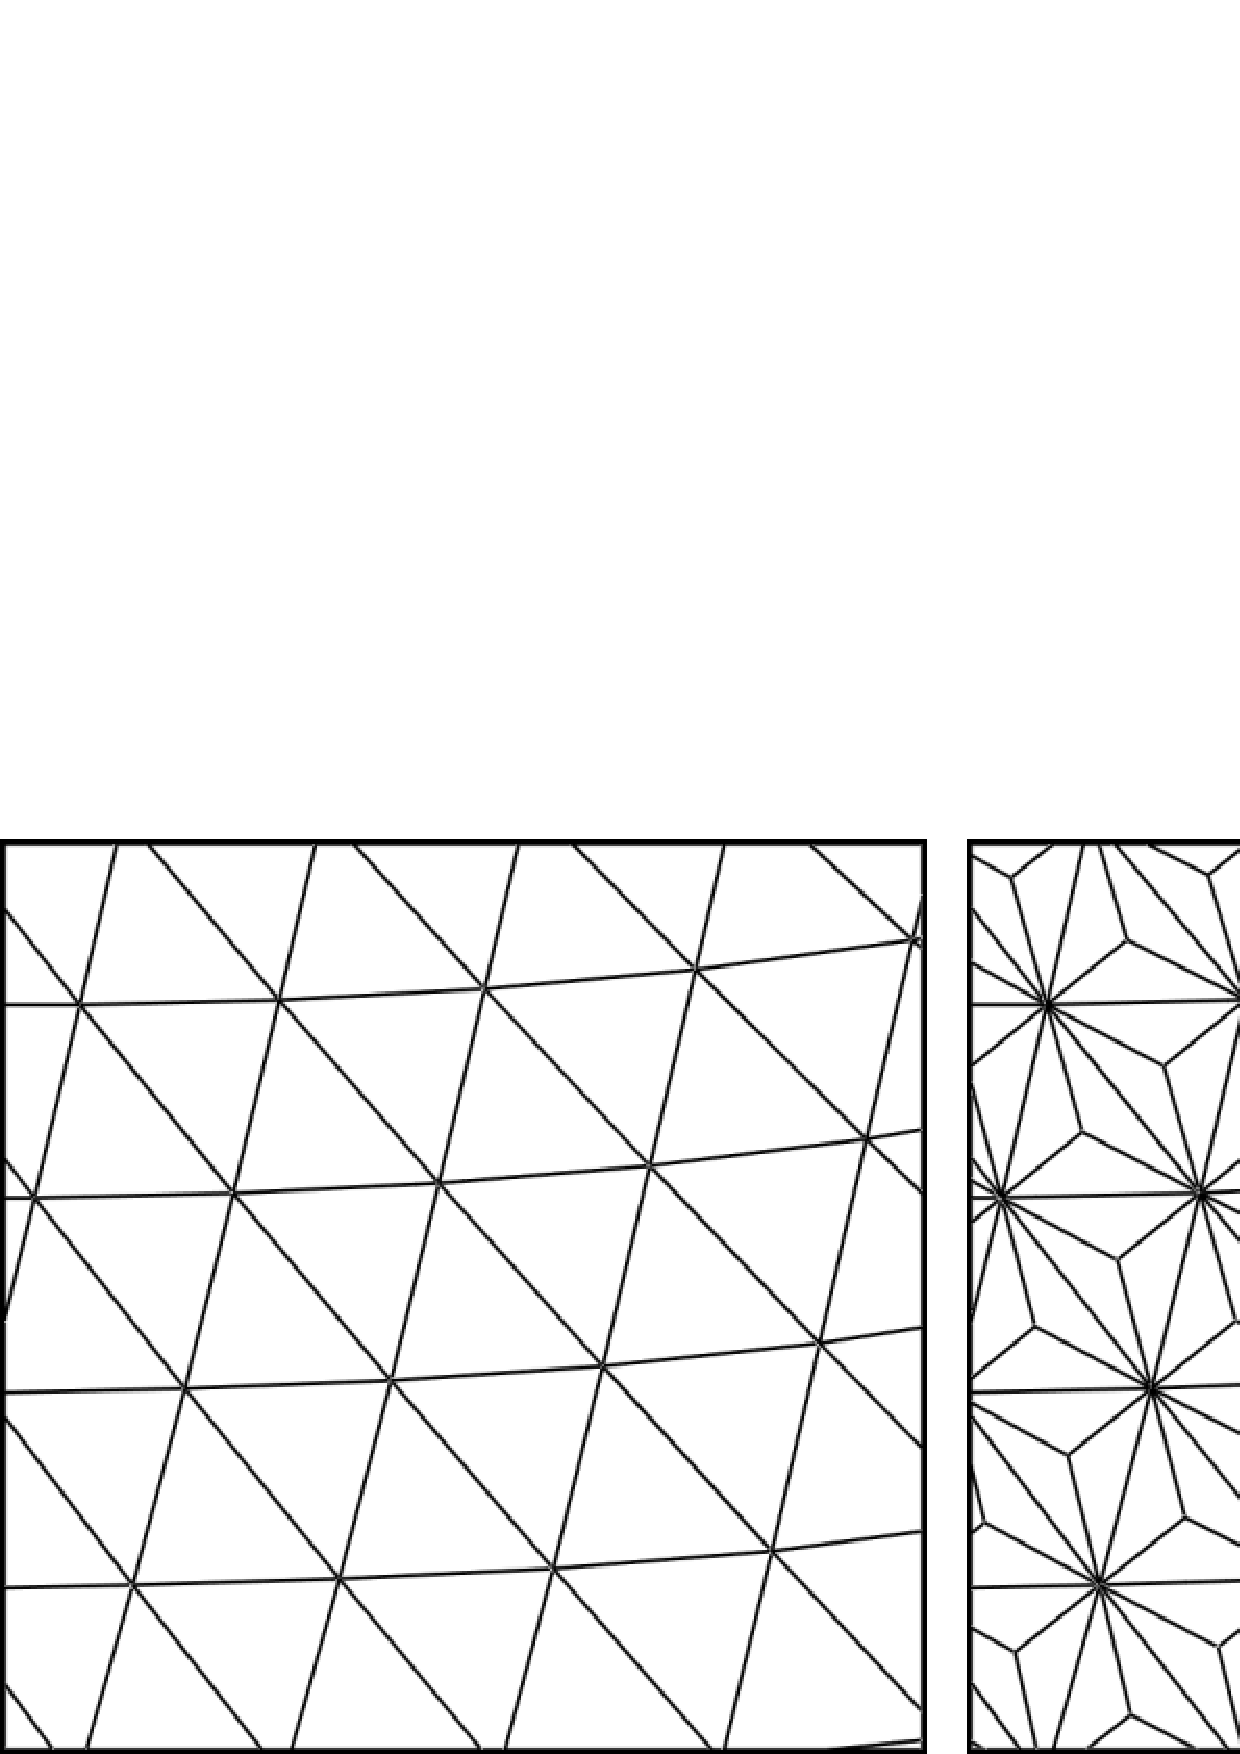
\includegraphics[width=7.0cm]{figs/sqrt3_basic}}
    \caption{The $\sqrt{3}$-Subdivision scheme is decomposed as
             a set of Euler operators: face splits and edge flips.}
    \label{fig:sqrt3_basic}
\end{figure}

\begin{figure}[htb]
    \centering{\includegraphics[width=7.0cm]{figs/sqrt3}}
    \caption{$\sqrt{3}$-Subdivision of the mannequin mesh.}
    \label{fig:sqrt3}
\end{figure}

\begin{tabular}{l|lll}
  \textbf{$\sqrt{3}$ subdivision} & \cgal\ float & \cgal\ double &
  \openmesh\ float \\\hline
  Lion vase: subdiv 1  & 0.95 & 1.22 &  1.27 \\
  Lion vase: subdiv 2  & 3.90 & 23.73 & 128 (swap)
\end{tabular}

\begin{tabular}{l|ll}
  \textbf{load OFF file} & \cgal (binary) & \openmesh (ascii) \\\hline
  Bunny     &  0.7 & 0.8\\
  Lion vase &  4.2 & 4.5 \\
  David     &  7.6 & 9.6 \\
  Raptor    &  22.0 7 20.6
\end{tabular}

